\documentclass[tikz]{standalone}
\usepackage{amsmath,amssymb}
\usetikzlibrary{arrows.meta}

% Classes of morphisms
\newcommand{\all}{\mathsf{all}}
\newcommand{\inj}{\mathsf{inj}}
\newcommand{\surj}{\mathsf{surj}}
\newcommand{\bij}{\mathsf{bij}}
\newcommand{\init}{\mathsf{init}}
\newcommand{\pb}{\mathsf{pb}}
\newcommand{\homog}{\mathsf{homog}}
\DeclareMathOperator{\id}{id}
\begin{document}
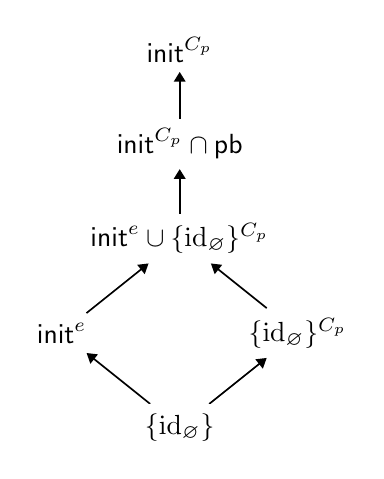
\begin{tikzpicture}[xscale=2,yscale=1.2]
\node (v0) at (0, -2) {$ \{\id_\varnothing\} $};
\node (v1) at (-0.75, -1) {$ \init^e $};
\node (v2) at (0.75, -1) {$ \{\id_\varnothing\}^{C_p} $};
\node (v3) at (0, 0) {$ \init^e \cup \{\id_\varnothing\}^{C_p} $};
\node (v4) at (0, 1) {$ \init^{C_p} \cap \pb $};
\node (v5) at (0, 2) {$ \init^{C_p} $};
\draw[white, ultra thick, double=black, arrows={-Triangle[black,scale=0.25]}] (v0) -- (v1);
\draw[white, ultra thick, double=black, arrows={-Triangle[black,scale=0.25]}] (v0) -- (v2);
\draw[white, ultra thick, double=black, arrows={-Triangle[black,scale=0.25]}] (v1) -- (v3);
\draw[white, ultra thick, double=black, arrows={-Triangle[black,scale=0.25]}] (v2) -- (v3);
\draw[white, ultra thick, double=black, arrows={-Triangle[black,scale=0.25]}] (v3) -- (v4);
\draw[white, ultra thick, double=black, arrows={-Triangle[black,scale=0.25]}] (v4) -- (v5);
\node[fill=white] at (v0) {$ \{\id_\varnothing\} $};
\node[fill=white] at (v1) {$ \init^e $};
\node[fill=white] at (v2) {$ \{\id_\varnothing\}^{C_p} $};
\node[fill=white] at (v3) {$ \init^e \cup \{\id_\varnothing\}^{C_p} $};
\node[fill=white] at (v4) {$ \init^{C_p} \cap \pb $};
\node[fill=white] at (v5) {$ \init^{C_p} $};
\end{tikzpicture}
\end{document}

